\chapter{Исследовательский раздел}
\section{Технические характеристики}
Технические характеристии устройства, на котором выполнялось тестирование:
\begin{itemize}
	\item операционная система: Windows 10 Pro;
	\item память: 8 GiB;
	\item процессор: Intel(R) Core(TM) i5-8265U CPU @ 1.60GHz   1.80 GHz.
\end{itemize}
Тестирование проводилось на ноутбуке, который был подключен к сети питания. Во время проведения тестирования ноутбук был нагружен только встроенными приложениями окружения, самим окружением и системой тестирования.

\section{Временные харастеристики выполнения}
Ниже был проведен анализ времени работы алгоритмов. Исходными данными является массив. Единичные замеры выдадут крайне маленький результат, поэтому  проведем работу каждого алгоритма n = 1000 раз и поделим на число n. Получим среднее значение работы каждого из алгоритмов. 

Выполним анализ для случая, когда массив целых чисел упорядочен по возрастанию. Результат приведен на рис \ref{fg:ref1}:

\begin{figure}[H]
	\centering{
		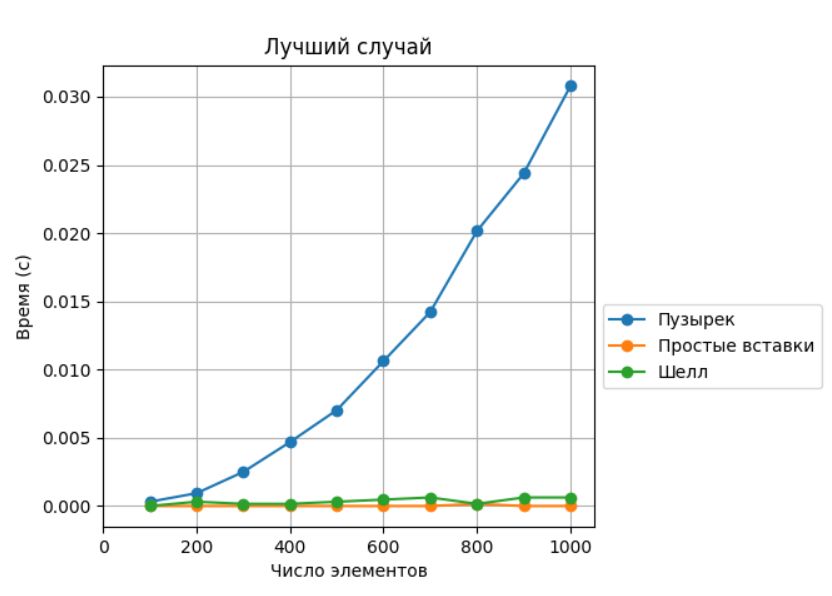
\includegraphics[width=10.6cm]{../../../../../../../msys64/home/Лев/bmstu_sem_5_aa/lab_03/report/images/1}
		\caption{Сравнение времени работы алгоритмов Левенштейна.}
		\label{fg:ref1}}
\end{figure} 

Как видно из результатов, алгоритм сортировки пузырьком работает медленне, чем сортировка вставкой или методом Шелла. Две последние сортировки работают примерно с одинаковой скоростью выполнения. 

Выполним анализ для случая, когда массив целых чисел имеет случайные значения. Результат приведен на рис. \ref{fg:ref2}:
\begin{figure}[H]
	\centering{
		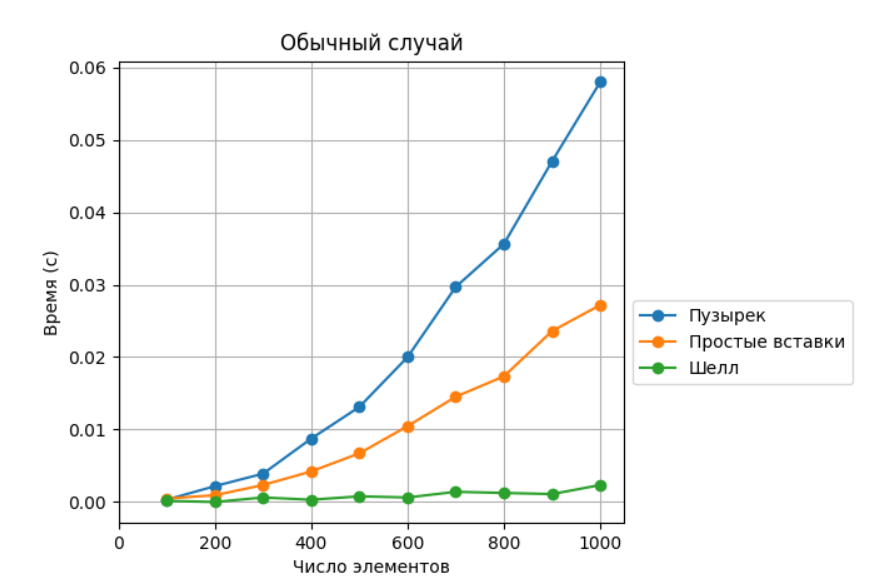
\includegraphics[width=10.6cm]{../../../../../../../msys64/home/Лев/bmstu_sem_5_aa/lab_03/report/images/2}
		\caption{Сравнение времени работы рекурсивного и некурсивного алгоритмов Левенштейна.}
		\label{fg:ref2}}
\end{figure}
Как видно из результатов алгоритм пузырька вновь работает медленнее двух остальных алгоритмов. Метод простых вставок уступает по скорости выполнения сортировки методу Шелла. 

Выполним анализ для случая, когда массив целых чисел отсортирован в обратном порядке. Результат приведен на рис.
\ref{fg:ref3}:
\begin{figure}[H]
	\centering{
		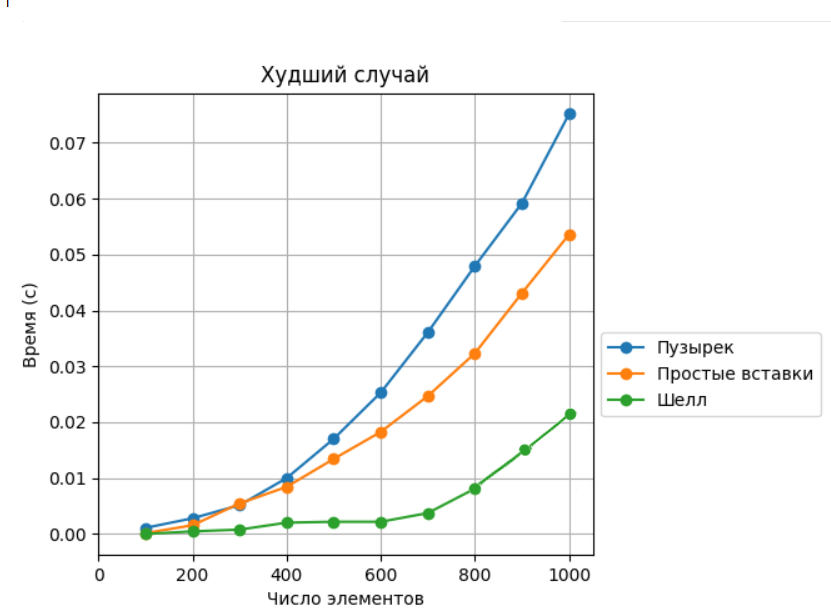
\includegraphics[width=10.6cm]{../../../../../../../msys64/home/Лев/bmstu_sem_5_aa/lab_03/report/images/3}
		\caption{Сравнение времени работы рекурсивного и некурсивного алгоритмов Левенштейна.}
		\label{fg:ref3}}
\end{figure} 

Как видно из результатов в данном случае алгоритм простых вставок работает медленее по сравнению с массивом, который имеет случайные целые числа. Метод Шелла уменьшил скорость выполнения по сравнению с предыдущим анализом времени выполнения. 

\section*{Вывод}
Алгоритм сортировки методом пузырька работает медленнее двух других рассмотренных алгоритмов, причем на больших размерах массива скорость выполнения этого алгоритма увеличивается значительно. Это проявляется также и при любом виде хранения целых чисел в массиве (упорядоченный, случайные числа, упорядоченный в обратном порядке).

Алгоритм сортировки простыми вставками работает также быстро, как и метод Шелла при упорядоченных данных в массиве. Метод Шелла работает значительно быстрее всех других приведенных алгоритмов, даже когда массив отсортирован в обратном порядке.